% Drawbotics Projekt Dokumentation
%
%
% Replaced "include" with "input" to make it work.
%%\input{stuff/header}
\documentclass
  [
  12pt                  % schriftgröße
  %twoside            % beidseitiger Druck
  , openright          % Kapitel beginnen auf einer rechten Seite
  , listof=totoc       % Verzeichnisse im Inhaltsverzeichnis
  , bibliography=totoc % Literaturverzeichnis im Inhaltsverzeichnis
  , parskip=half       % Absätze durch einen vergrößerten Zeilenabstand getrennt
%  , draft              % Entwurfsversion
  ]{scrreprt}          % Dokumentenklasse: KOMA-Script Buch
  

%%%%%%%%%%%%%%%%%%%%%%%%%%%%%%%%%%%%%%%%%%%%%%%%%%%%%%%%%%%%%%%%%%%%%%%
% Packages
%%%%%%%%%%%%%%%%%%%%%%%%%%%%%%%%%%%%%%%%%%%%%%%%%%%%%%%%%%%%%%%%%%%%%%%
\usepackage{scrhack}

 
\usepackage{ifpdf}
\ifpdf
  \usepackage{ae}               % Fonts für pdfLaTeX, falls keine cm-super-Fonts installiert
  \usepackage{microtype}        % optischer Randausgleich, falls pdflatex verwandt
  \usepackage[pdftex]{graphicx} % Grafiken in pdfLaTeX
\else
  \usepackage[dvips]{graphicx}  % Grafiken und normales LaTeX
\fi

\usepackage[a4paper,%
            inner=2.0cm,outer=2.0cm,bindingoffset=0.5cm,%
            top=1.5cm,bottom=1.5cm,%
            footskip=1.0cm,includeheadfoot]{geometry}
            
\usepackage[utf8]{inputenc}         % Input encoding (allow direct use of special characters like "ä")
%\usepackage[english]{babel}
\usepackage[ngerman]{babel}
\usepackage[T1]{fontenc}
\usepackage[automark]{scrpage2} 	 % Schickerer Satzspiegel mit KOMA-Script
\usepackage{setspace}           	 % Allow the modification of the space between lines
\usepackage{booktabs}           	 % Netteres Tabellenlayout
\usepackage{multicol}               % Mehrspaltige Bereiche
\usepackage{quotchap}               % Beautiful chapter decoration
\usepackage[printonlyused]{acronym} % list of acronyms and abbreviations
\usepackage{subfig}                 % allow sub figures
\usepackage{tabularx}               % Tabellen mit fester Breite
\usepackage{lipsum}                 % für Blindtexte
\usepackage[addtotoc]{abstract}
\usepackage{easyfig}				% Bilder einfach einbinden
\usepackage{array,multirow}
\usepackage{float}
\usepackage{amsmath}
\usepackage{amssymb}

% Layout
\pagestyle{scrheadings}
%\pagestyle{empty}
\clubpenalty = 10000
\widowpenalty = 10000
\displaywidowpenalty = 10000

\makeatletter
\renewcommand{\fps@figure}{htbp}
\makeatother

%% Document properties %%%%%%%%%%%%%%%%%%%%%%%%%%%%%%%%%%%%%%%%%%%%%%%%
\newcommand{\titel}{Eliptic Curve Digital Signature Algorithm}
\newcommand{\thesisname}{Reconfigurable Computing}
\newcommand{\untertitel}{FPGA-Implementierung und Vergleich}
\newcommand{\Datum}{23. November 2017}

\ifpdf
  \usepackage{hyperref}
  \definecolor{darkblue}{rgb}{0,0,.5}
  \hypersetup
  	{ colorlinks=true
  	, breaklinks=true
    , linkcolor=darkblue
    , menucolor=darkblue
    , urlcolor=darkblue
    , citecolor=darkblue
    , pdftitle={\title -- \untertitel}
    , pdfsubject={\thesisname}
    , pdfauthor={Sawitzki, Bublies, Schulz}
    }
\else
\fi

\bibliographystyle{alpha}

%% Listings %%%%%%%%%%%%%%%%%%%%%%%%%%%%%%%%%%%%%%%%%%%%%%%%%%%%%%%%%
\usepackage{listings}
\KOMAoptions{listof=totoc} % necessary because of scrhack
\renewcommand{\lstlistlistingname}{List of Listings}
\lstset
  { basicstyle=\small\ttfamily
  , breaklines=true
  , captionpos=b
  , showstringspaces=false
  , keywordstyle={}
  }

\lstnewenvironment{inlinehaskell}
{\spacing{1}\lstset{language=haskell,nolol,aboveskip=\bigskipamount}}
{\endspacing}

\lstnewenvironment{inlinexml}
{\spacing{1}\lstset{language=XML,nolol,aboveskip=\bigskipamount}}
{\endspacing}

\newcommand{\haskellinput}[2][]{
  \begin{spacing}{1}
  \lstinputlisting[language=Haskell,nolol,aboveskip=\bigskipamount,#1]{#2}
  \end{spacing}
}

\newcommand{\haskellcode}[2][]{\mylisting[#1,language=Haskell]{#2}}

\newcommand{\mylisting}[2][]{
\begin{spacing}{1}
\lstinputlisting[frame=lines,aboveskip=2\bigskipamount,#1]{#2}
\end{spacing}
}

\begin{document}

\pagenumbering{Roman}

%%%%%%%%%%%%%%%%%%%%%%%%%%%%%%%%%%%%%%%%%%%%%%%%%%%%%%%%%%%%%%%%%%%
%%%%%%%%%%%%%%%%%%%%%%%%%%%%%%%%%%%%%%%%%%%%%%%%%%%%%%%%%%%%%%%%%%%
%%%%%%%%%%%%%%%%%%%%%%%%%%%%%%%%%%%%%%%%%%%%%%%%%%%%%%%%%%%%%%%%%%%
%%%%%%%%%%%%%%%%%%%%%%%%%%%%%%%%%%%%%%%%%%%%%%%%%%%%%%%%%%%%%%%%%%%
%%%%%%%%%%%%%%%%%%%%%%%%%%%%%%%%%%%%%%%%%%%%%%%%%%%%%%%%%%%%%%%%%%%


% Titelseite
%!TEX root = ../thesis.tex

\titlehead{
  \centering
  
\includegraphics[width=.5\textwidth]{bilder/fhw}\\
  \bigskip
  \textsc{\Large Department of Computer Science}
}

\subject{\thesisname}
\title{\titel}
\subtitle{\Large \untertitel}
\date{\vspace{-1cm}{\small Eingereicht am:}\\\medskip\Datum}
\author{}
\publishers{\vfill
  \normalsize
  \begin{minipage}{13cm}

    \bigskip
    %\bigskip
       
    \begin{multicols}{2}
      \raggedright
	  
      \vspace{1cm}
      {\Large Lennart Bublies}
      {\small inf100434@fh-wedel.de}\\
      \vspace{0.8cm}
      
      {\Large Leander Schulz}
      {\small inf102143@fh-wedel.de}\\
      \vspace{0.3cm}
      
      \raggedleft
      
      {\small Betreut von:}\\
      \smallskip
      {\Large Prof. Dr. S. Sawitzki}\\
      \vspace{0.3cm}
      Fachhochschule Wedel\\
      Feldstraße 143\\
      22880 Wedel\\
      %Phone: (041\,03)~80\,48-41\\
      E-mail: saw@fh-wedel.de\\
    \end{multicols}
 \end{minipage}
}

\uppertitleback{
  {\huge \titel}\bigskip\\  
  {\Large \untertitel}\bigskip\\
  {\large \thesisname von \authorname}
  \begin{abstract}
  Das ist ein Einleitungstext!
  \end{abstract}
}

\lowertitleback{

Copyright {\small \copyright} 2011 \authorname \bigskip\\
Irgendein Copyright Text
Layout done with {\rmfamily \LaTeXe}, {\sffamily \KOMAScript} and {\rmfamily B\textsc{ib}\TeX}.
}

\maketitle




%%%%%%%%%%%%%%%%%%%%%%%%%%%%%%%%%%%%%%%%%%%%%%%%%%%%%%%%%%%%%%%%%%%
%%%%%%%%%%%%%%%%%%%%%%%%%%%%%%%%%%%%%%%%%%%%%%%%%%%%%%%%%%%%%%%%%%%
%%%%%%%%%%%%%%%%%%%%%%%%%%%%%%%%%%%%%%%%%%%%%%%%%%%%%%%%%%%%%%%%%%%
%%%%%%%%%%%%%%%%%%%%%%%%%%%%%%%%%%%%%%%%%%%%%%%%%%%%%%%%%%%%%%%%%%%
%%%%%%%%%%%%%%%%%%%%%%%%%%%%%%%%%%%%%%%%%%%%%%%%%%%%%%%%%%%%%%%%%%%

% abstract
\renewcommand{\abstractname}{Abstract}
\begin{abstract}
\vspace{0.5cm}
\begin{center}
\begin{minipage}[h]{0.8\textwidth}

In this work....

    
\end{minipage}
\end{center}    
\end{abstract}


\newpage
%%%%%%%%%%%%%%%%%%%%%%%%%%%%%%%%%%%%%%%%%%%%%%%%%%%%%%%%%%%%%%%%%%%%%%%
\renewcommand{\abstractname}{Zusammenfassung}
\begin{abstract}
\vspace{0.5cm}
\begin{center}
\begin{minipage}[h]{0.8\textwidth}

% Ausgangslage
In dieser Arbeit wird ein Algorithmus zur Erstellung und Überprüfung digitaler Signaturen für den Betrieb auf einem FPGA implementiert. Die gemessene Performance der Hardware wird 

% Vorgang, Inhalt


% Ergebnis



\end{minipage}
\end{center}

\end{abstract}
\newpage
\tableofcontents
\cleardoublepage


\pagenumbering{arabic}

\onehalfspacing

%!TEX root=../ecdsa.tex
% \lipsum
\chapter{Einleitung}
Mit wachsender Digitalisierung wächst auch die Sorge, was mit den eigenen Daten passiert und ob diese nach der Übertragung über ein Medium nicht durch andere manipuliert worden sind. Um die Sicherheit bzw. Authentizität der Daten zu gewährleisten, werden die Daten mit Hilfe eines Passwortes, dem Schlüssel, signiert, sodass ein Empfänger, der ebenfalls den Schlüssel kennt, die Daten verifizieren kann. Der sich dahinter verbergende Algorithmus wird Digitaler Signatur Algorithmus (engl. Digital Signature Algorithm, DSA) genannt.
\\ \\
Will ein Angreifer trotz Signatur eine Nachricht manipulieren, kann dieser über eine Brute-Force-Attacke versuchen, den Schlüssel durch ein Testen jeder erdenklichen Kombination zu erraten. Gelingt dies, kann nach der Manipulation eine neue gültige Signatur erstellt werden. Um diesem Angriffsszenario entgegen zu wirken, werden lange Schlüssel verwendet, sodass eine solche Attacke nicht in akzeptabler Zeit zu bewerkstelligen ist. Dies hat jedoch zur Folge, dass mit steigender Schlüssellänge auch die Zeit steigt, die für das Erstellen der Signatar bzw. die Verifizierung benötigt wird. 
\\ \\
Eine mögliche Lösung zur Reduzierung der Schlüssellänge und damit der Laufzeit besteht im Einsatz optimierter Verfahren wie die elliptischen Kurven, die im Gegensatz zu Verfahren wie RSA (engl. Random Sequential Adsorption), deutlich geringe Schlüssellängen benötigen. Diese Arbeit widmet sich den zuvor erwähnten elliptischen Kurven mit dem Ziel, eine effiziente Hardware-Implementierung zu entwickeln, die eine klassische Software-Variante übertrifft.

%!TEX root=../ecdsa.tex

\chapter{Zielsetzung \& Abgrenzung} 
\label{sec:planung}
Das Ziel dieser Arbeit ist die Umsetzung eines kryptografisch sicheren Verfahrens zum digitalen Signieren einer Nachricht und der Verifikation dieser Signatur. Dazu dient der \textit{Elliptic Curve Digital Signature Algorithm (ECDSA)} als Basis, um eine ressourceneffiziente Hardware-Implementierung unter Verwendung eines FPGA-Bausteins\footnote{Field Programmable Gate Array (FPGA): https://de.wikipedia.org/wiki/Field\_Programmable\_Gate\_Array} zu implementieren. Als Entwicklerboard kommt das Altera DE2 Board zum Einsatz. 
\\ \\
Die Kommunikation mit dem FPGA soll über eine serielle Schnittstelle erfolgen. Dabei gibt es die zwei Modi Signieren und Verifizieren. Beim Signieren wird die zu signierende Nachricht gesendet und als Antwort eine gültige Signatur empfangen. Beim Verifizieren werden die zu überprüfende Signatur und die Originalnachricht gesendet. Als Antwort wird über einen booleschen Wert signalisiert, ob die Signatur gültig ist oder nicht. Dabei liegt der Fokus auf der VHDL-Implementierung der mathematischen Funktionen und der Lauffähigkeit des Gesamtsystems. Auf Teilkomponenten wie die Generierung einer echten Zufallszahl oder die effiziente Bildung eines Hashes der Nachricht, wie im Algorithmus beschrieben, wird verzichtet. Stattdessen werden die Daten bereits als Hash übertragen und eine Konstante als Zufallszahl verwendet. An dieser Stelle sei erwähnt, dass das Verwenden einer Konstante als Zufallszahl kryptografisch unsicher ist und in produktiven Umgebungen zwingend vermieden werden sollte, um Angriffe wie den berühmten Playstation 3 Hack\footnote{Playstation 3 Hack: https://www.edn.com/design/consumer/4368066/The-Sony-PlayStation-3-hack-deciphered-what-consumer-electronics-designers-can-learn-from-the-failure-to-protect-a-billion-dollar-product-ecosystem} zu verhinden. Neben der Konstante werden alle weiteren benötigten Parameter der ECDSA-Implementierung als gegeben vorausgesetzt und fest verdrahtet. Die Vereinfachungen sind zum einen der fehlenden Hardware zur Generierung einer echten Zufallszahl geschuldet und zum anderen um den Fokus auf die Implementierung der Kernfunktionen zu lenken.  
\\ \\
Abgeschlossen wird diese Arbeit mit einer Gegenüberstellung der Ergebnisse der FPGA-Implementierung mit einer C-Implementierung, die im Rahmen eines anderen Projektes \cite{kewish} entstanden ist.


%%%%%%%%%%%%%%%%%%%%%%%%%%%%%%%%%%%%%%%%%%%%%%%%%%%%%%%%%%%%%
%\section{Problemanalyse}
%Bevor mit der Implementierung des ECDSA-Algorithmus begonnen wird, gilt es %zunächst die Aufgabenstellung präzise zu erfassen. Dazu müssen die %theoretischen Grundlagen und zugrunde liegenden Konzepte der zu verwendenden %Technologien erarbeitet werden. In Kapitel \ref{sec:basics} werden dazu die %wesentlichen mathematischen Grundlagen erläutert. 
%\\ \\
% ell kurve, galois felder -> komplizierter
%Beim ECDSA-Algorithmus kommen im Gegensatz zu klassischen Signaturverfahren, welche ebenso auf asymmetrischer Verschlüsselung basieren, Polynome elliptischer Kurven zum Einsatz. Um diese Funktionen in der Kryptografie einsetzen zu können, müssen Berechnungen in abgeschlossenen Räumen stattfinden. Hierzu wird ein Galois-Körper über der elliptischen Kurve definiert und die dazugehörigen Funktionen analysiert und in VHDL implementiert.
%!TEX root = ../thesis.tex

\chapter{Grundlagen} \label{sec:basics}

In diesem Kapitel werden die mathematischen Grundlagen erläutert und die wesentlichen Konzepte hinter dem behandelten Verschlüsselungs-Algorithmus beschrieben. \\

%%%%%%%%%%%%%%%%%%%%%%%%%%%%%%%%%%%%%%%%%%%%%%%%%%%%%%%%%%%%%
\section{Gruppen und Endliche Körper}

Eine abelsche Gruppe im mathematischen Sinn ist ein Tupel $(G,\circ)$ aus einer nicht-leeren Menge G und einer darauf definierten inneren Verknüpfung $\circ$ (vgl. \cite{puttmann}, S. 11f). Hierbei entspricht die innere Verknüpfung einer Abbildung 
\begin{center}
$ \circ: X \times X \to X $
\end{center}
die jedem Paar $(x_1,x_2)$ aus Elementen der Menge X ein Element $x_1 \circ x_2$ zuordnet. Außerdem sind folgende Bedingungen auf der Struktur einer Gruppe definiert: \\

\begin{enumerate}
  \item Menge $G$ ist abgeschlossen, d.h. für alle $a,b \in G$ gilt, d.h. dass auch jede Verknüpfung $a \circ b$ ein Element von $G$ ist. 
  \item Assoziativgesetz: $ \forall a,b,c \in G: (a \circ b) \circ c = a \circ (b \circ c) $
  \item Kommutativgesetz: $ \forall a,b \in G: a \circ b = b \circ a $
  \item Neutrales Element: $ \forall a \in G: a \circ e = e \circ a = a$
  \item Inverses Element: $ \forall a \in G: a \circ a^{-1} = a^{-1} \circ a = e$\\
\end{enumerate}

Ein Beispiel für eine so definierte abelsche Gruppe entspricht der Menge der ganzen Zahlen $\mathbb{Z}$ mit der Addition als Verknüpfung $(\mathbb{Z},+)$. Die Anzahl der Elemente einer Gruppe wird als Ordnung bezeichnet, welche für die ganzen Zahlen unendlich ist. In der Kryptographie kommen jedoch stets Gruppen mit einer endlichen Anzahl von Elementen zum Einsatz, bei denen also die Ordnung der Gruppe beschränkt ist. \\

Eine besondere Form endlicher Gruppen bilden zyklische Gruppen, die ein Element $g$ besitzen, aus dem durch Verknüpfungen $\circ$ alle anderen Elemente der Gruppe erzeugt werden können. Das Element $g$ ist das sog. Generatorelement der zyklischen Gruppe $(G',\circ)$. \\ 

Eine Körper ist eine Erweiterung von abelschen Gruppen und als Tripel $(K,+,\cdot)$ definiert, welche zu einer nicht-leeren Menge $K$ konkret die inneren Verknüpfungen Addition und Multiplikation beschreibt. Folgende Bedingungen werden dabei erfüllt (vgl. \cite{puttmann}):

\begin{enumerate}
  \item Die Menge $K$ bildet durch die additive Verknüpfung $+$ eine abelsche Gruppe
mit 0 als neutralem Element
  \item Die Menge $K\setminus\{0\}$, d. h. $K$ ohne das Element 0, bildet durch die multiplikative Verknüpfung $\cdot$ ebenfalls eine abelsche Gruppe mit 1 als neutralem Element
  \item Distributivgesetz: $ \forall a,b,c \in K: c \cdot (a + b) = c \cdot a + c \cdot b $
\end{enumerate}

Unter einem Endlichen Körper\footnote{auch: Galoiskörper, finites Feld} versteht man einen Körper mit endlich vielen Elementen, der oft auch als Restklassenkörper bezeichnet wird. Ein Beispiel dafür sind Primkörper mit Primzahl $p$ und den Verknüpfungen \textit{Addition modulo p} und \textit{Multiplikation modulo p}: $\mathbb{Z}_p = \{0,1,2,3,\cdots,p-1\}$. \\

Galoiskörper werden mit $GF(p)$ abgekürzt, wobei $q$ eine Primzahl sein muss und für die Anzahl der Elemente im Feld steht. $GF(p)$ repräsentiert damit einen Körper der Restklasse ganzer Zahlen modulo $p$. Durch die mathematischen Eigenschaften dieser Struktur um Restklassen und inverse Elemente eignen sie sich besonders für den Einsatz in der Kryptographie. \\


%%%%%%%%%%%%%%%%%%%%%%%%%%%%%%%%%%%%%%%%%%%%%%%%%%%%%%%%%%%%%
\section{Elliptische Kurven} \label{sec:ell}

Eine elliptische Kurve $E$ über einem Körper $K$ ist eine nicht-singuläre\footnote{keine Knoten, keine Spitzen, keine ``Einsiedler'' (isolierte Punkte)} Kurve (vgl. Abb. \ref{fig:ellkurve}), definiert als Menge aller Punkte $(x,y)$ mit $x,y \in K$, für die gilt $F(x,y)=0$ zusammen mit einem ``Punkt in der Unendlichkeit'' O (vgl. \cite{grebe}, S.25). \\

Eine elliptische Kurve über ein finites Feld $F_p$ kann mit Hilfe der Weierstraß-Gleichung in Normalform wie folgt definiert werden:

% E:y2+a1xy+a3 y=x3+a2x2+a4x+a6
\begin{center}
$E(K): y^2 + a_1 x y + a_3 y = x^3 + a_2 x^2 + a_4 x + a_6 $
\end{center}

Die Parameter $a_1 \dots a_6$ legen fest, welche Form die elliptische Kurve annimmt und sind Elemente des finiten Feldes $F_p$. Sie werden durch die Domain-Parameter festgelegt. 

\begin{figure}[H]
	\centering
   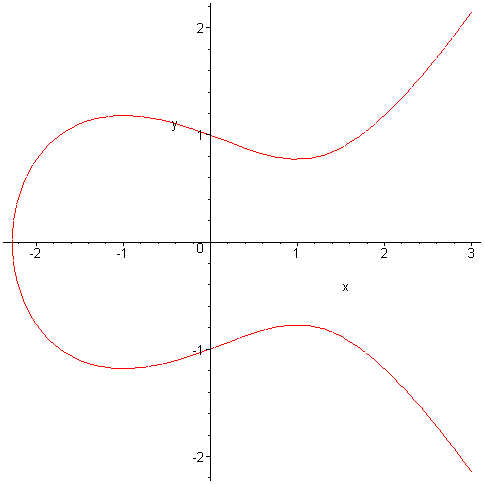
\includegraphics[width=0.60\textwidth]{bilder/ellkurve}
	\caption{Graph einer Elliptischen Kurve}
	\label{fig:ellkurve}
\end{figure}

Über eine Reihe von Vereinfachungen lässt sich die Weierstraß-Gleichung auf die folgende Formel reduzieren:  % y2 mod p=x3+ax+b mod p 
\begin{center}
$ y^2 \bmod p = x^3 + a x + b \bmod p $
\end{center}


Damit eine elliptische Formel in der Kryptographie eingesetzt werden kann, muss zusätzlich nachfolgende Bedingung gelten. Sie folgt aus der nicht-singulären Eigenschaft von E, also Ableitungen $\ne$ 0 und bzw. Diskriminante $\ne$ 0 (Herleitung und Beweis siehe \cite{grebe}, S. 28ff):
%4a3+ 27b2 mod p 0
\begin{center}
$ 4 a^3 + 27 b^2 \bmod p \ne 0, $ mit $ a,b \in K $
\end{center}

Entsprechend wie bei endlichen Körpern ist die Ordnung auf einer zyklischen Untergruppe $U_P$ von $E(F_P)$ definiert (vgl. \cite{grebe}, S. 35):
\begin{center}
$ U_P := \{ k P | k \in \mathbb{Z} \}$
$k_0 P = P + P + \cdots + P = O, $ mit $ k_0 > 0$
\end{center}

Die als Punktaddition bezeichnete arithmetische Operation verknüpft zwei verschiedene Punkte ($P_1 \ne P_2$) auf der Kurve miteinander. Wenn die beiden Punkte gleich sind (also $P_3 = P_1 + P_2 = 2 P_1$), wird diese Operation Punktverdopplung genannt (vgl. \cite{puttmann}, S. 16f). Beide Operationen lassen sich mittels Sekanten- bzw. Tangentenmethode auf einer elliptischen Kurve darstellen (s. Abb. \ref{fig:padd}). 

\begin{figure}[H]
	\centering
   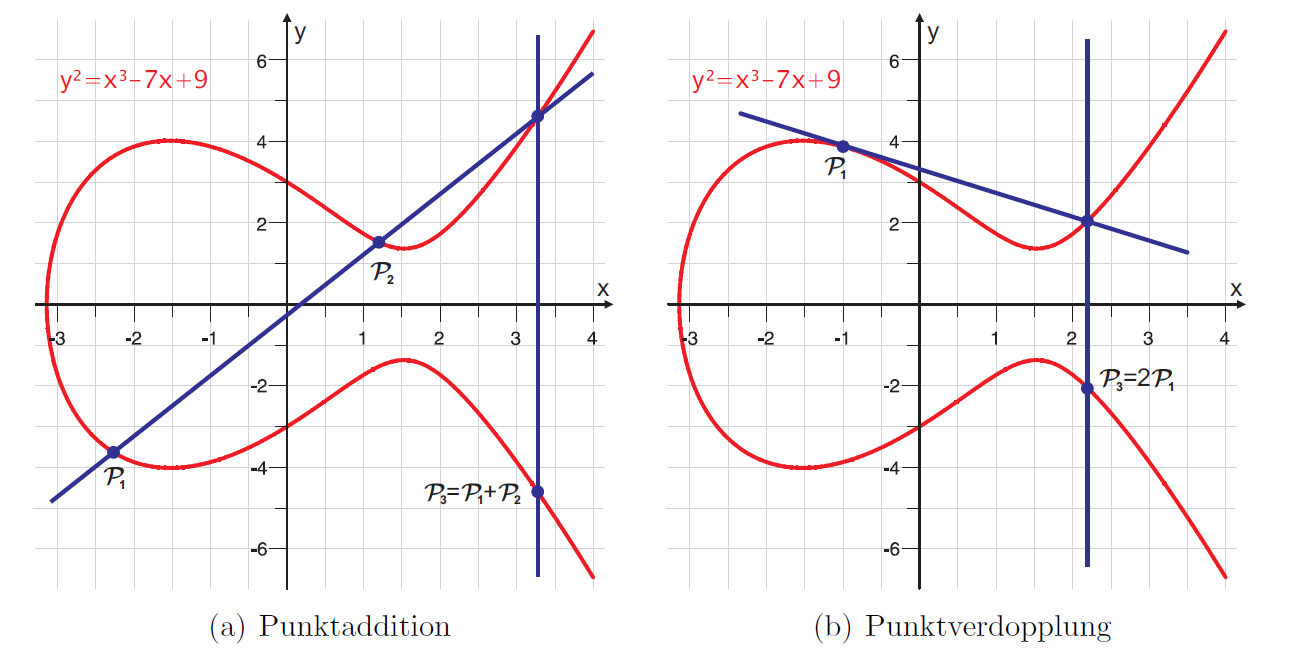
\includegraphics[width=\textwidth]{bilder/p-addition}
	\caption{Arithmetische Operationen auf einer elliptischen Kurve}
	\label{fig:padd}
\end{figure}

Eine besondere Form der elliptischen Kurven sind \texttt{Koblitz}-Kurven\footnote{engl.: Anomalous Binary Curves} über $F_{2^m}$, deren Kurvengleichung ausschließlich die Koeffizienten ``0'' und ``1'' enthalten. In kryptographischen Protokollen werden häufig Koblitz-Kurven der folgenden Formen verwendet (vgl. \cite{guide}, Kap. 3.4): \\
\begin{center}
$E_0 : y^2 + x y = x^3 + 1 $ \\
$E_1 : y^2 + x y = x^3 + x^2 + 1 $
\end{center}

Der große Vorteil dieser Kurven ist, dass Algorithmen zur Punktmultiplikation prinzipiell ohne Punktverdopplung auskommen können (s. \cite{guide}, S. 114).
Koblitz-Kurven besonders für den Einsatz in Hardwaresystemen geeignet, da für sie allgemein hocheffiziente Algorithmen für Punktarithmetik existieren, wohingegen klassische Kurven $F_P$ eher für Softwaresysteme eignen. In der Praxis wurden bisher keine Sicherheitsunterschiede festgestellt. \\


%%%%%%%%%%%%%%%%%%%%%%%%%%%%%%%%%%%%%%%%%%%%%%%%%%%%%%%%%%%%%
\section{Das Diskrete Logarithmus-Problem} \label{sec:dlp}

Das Problem des diskreten Logarithmus in endlichen Körpern besteht darin, dass die Lösung eines solchen Logarithmus viel schwieriger ist als die Umkehrfunktion, also die diskrete Exponentialfunktion. Die Sicherheit von auf elliptischen Kurven basierenden kryptographischen Verfahren beruht auf diesem mathematischen Problem. \\

Definition nach \cite{baum} (S. 6):
\begin{itemize}
	\item \textbf{Voraussetzungen:}\\
	Sei $(G,\cdot)$ eine multiplikative Gruppe, $x \in G$ ein Element der Ordnung $n$ und $y \in \left \langle x \right \rangle$. \\
	\item \textbf{Problem:}\\
	Man berechnet $a$ mit $(0 \le a \le n-1)$, sodass $x^a = y$. \\
	``$a$'' wird diskreter Logarithmus von $y$ zur Basis $x$ genannt. \\
\end{itemize}

Umgangssprachlich wird eine solche Funktion \textit{Einwegfunktion} genannt. Dabei entspricht der diskrete Logarithmus einer Funktion $f: M \implies N$, wenn für ``fast alle'' Bilder $y \in N$ kein Urbild $x \in M$ mit $f(x) = y$ effizient bestimmbar ist (vgl. \cite{diskrlog}, S. 54). \\

Bezogen auf eine elliptische Kurve\footnote{engl. elliptic curve discrete logarithm problem (ECDLP)} $E(GF(2^n))$ bedeutet das, dass die Skalarmultiplikation $Q = k P$ für eine natürliche Zahl $k$ und einen Punkt $P$ nach der Kurvengleichung in Kap. \ref{sec:ell} sehr einfach zu berechnen ist ($Q$ ist die $(k-1)$-fache Addition mit $P$), es aber \textit{schwierig} ist, aus zwei vorgegebenen Punkten $Q, P \in E(GF(2^n))$ wieder die Zahl $k$ zu ermitteln (vgl. \cite{puttmann}, S. 17f). \\


%%%%%%%%%%%%%%%%%%%%%%%%%%%%%%%%%%%%%%%%%%%%%%%%%%%%%%%%%%%%%
\section{Digitale Signaturen} \label{sec:digsig}

Eine digitale Signatur nutzt ein asymmetrischen Verschlüsselungsverfahren, um eine schlüsselabhängige Prüfsumme anhand eines Dokuments\footnote{In der Praxis wird aus Performanz-Gründen oft ein Hash der Nachricht bzw. des Dokuments verwendet.} in Kombination mit einem Schlüssel zu erzeugen (vgl. \cite{wolf}). ``Der Schlüssel zum Überprüfen einer Signatur ist öffentlich, während der Schlüssel zum Signieren geheim gehalten werden muß.'' Somit kann jeder ein digital ``unterschriebenes'' Dokument auf seine Echtheit überprüfen, also \textit{verifizieren}. \\

\begin{figure}[H]
	\centering
   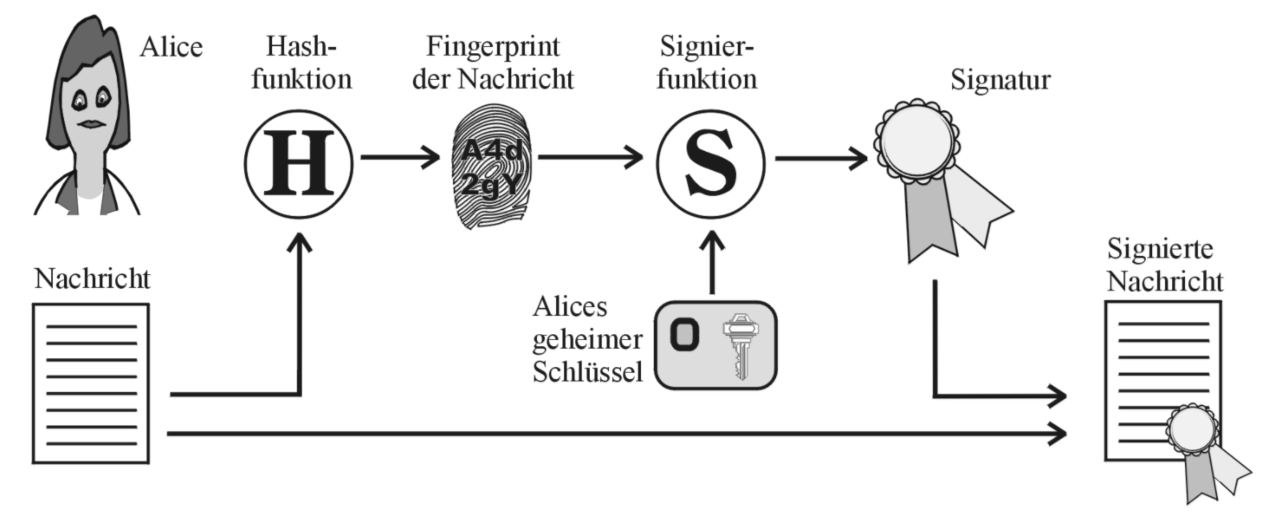
\includegraphics[width=0.80\textwidth]{bilder/digisig}
	\caption{Erzeugung einer Digitalen Signatur}
	\label{fig:digisig}
\end{figure}

Abbildung \ref{fig:digisig} zeigt den Vorgang der Erzeugung einer Signatur. Die im Bild zu sehende ``Signierfunktion'' muss eine asymmetrische Verschlüsselung sein und entspricht dem in dieser Arbeit implementierten ECDSA-Algorithmus. \\

%%%%%%%%%%%%%%%%%%%%%%%%%%%%%%%%%%%%%%%%%%%%%%%%%%%%%%%%%%%%%
\section{Der ECDSA}

%Beim \textit{Elliptic Curve Digital Signature Algorithm} ist die Multiplikation mit einem Punkt auf der elliptischen Kurve die rechnerisch aufwändigste Operation (vgl. \cite{hwimp}), genauer die Skalarmultiplikation $k P$, wobei $k$ eine positive Ganzzahl und $P$ ein Punkt auf der Kurve ist. \\

\subsection{Schlüsselgenerierung \& Domain Parameter}

Beim \textit{Elliptic Curve Digital Signature Algorithm} wird von einer Partei A ein Schlüssel generiert und damit die Signatur zu einer Nachricht erstellt. Eine andere Partei B nutzt den öffentlichen Schlüssel von A und verifiziert damit die Echtheit der Nachricht von A anhand der Signatur. Folgende Definition (vgl. \cite{hwimp}) berechnet die Schlüssel von A: \\

\begin{enumerate}
%Key generation : (A)
\item Wähle ein zufälliges $d$ aus $[1, n-1]$.
\item Berechne $Q = dP$ .
\item Der Public Key von A entspricht $Q$; der Private Key ist $d$. \\
\end{enumerate}

Der private Schlüssel $d$ ist hierbei eine positive ganze Zahl. Der Parameter $n$ entspricht der Ordnung des Basis-Punkts $P$. In der Hardware-Implementierung dieser Arbeit wird für den Private Key stets ein konstanter Wert verwendet, da der Fokus auf dem ECDS-Algorithmus liegt und nicht auf dem Finden einer echten Zufallszahl. \\

Die Domain Parameter werden allgemein angegeben als $D = (q,FR, S,a,b, P,n,h)$ und werden definiert als (vgl. \cite{guide}, S. 172):
\begin{itemize}
\item $q$: Ordnung der Kurve.
\item $FR$: \textit{field representation}, Repräsentation der Elemente in $F_q$.
\item $S$: \textit{Seed}, falls die Kurve zufällig generiert ist.
\item $a,b \in F_q$: Koeffizienten, die die elliptische Kurve beschreiben.
\item $P = (x_P,y_P) \in E(F_q)$: Basis-Punkt der elliptischen Kurve.
\item $n$: Ordnung von $P$.
\item $h$: \textit{Ko-Faktor} $h = \#E(F_q)/n$.
\end{itemize}

\subsection{Signatur}

Die Signatur wird nach folgendem Vorgehen erstellt (vgl. \cite{hwimp}):\\

Signature generation : (A)
\begin{enumerate}
\item Select a random integer $k$ from $[1, n - 1]$.
\item Compute $k G = (x_1, y_1)$ and $r = x_1 \pmod{n} $.
\item If $r = 0$ then go to step 1.
\item Compute $k^{-1} \pmod{n}$.
\item Compute $s = k^{-1}(SHA - 1(m) + dr)\pmod{n}$.
\item If $s = 0$ then go to step 1.
\item Send $m$ and $(r, s)$, which is A’s signature for the message $m$, to B.
\end{enumerate}

\subsection{Verifikation}

Die Verifikation wird nach folgendem Vorgehen durchgeführt (vgl. \cite{hwimp}):\\

Signature verification : (B)
\begin{enumerate}
\item Verify that $r$ and $s$ are integers in $[1, n - 1]$.
\item Compute $e = SHA - 1(m)$.
\item Compute $w = s^{-1}\pmod{n}$.
\item Compute $u_1 = e * w \pmod{n}$ and $u_2 = r * w \pmod{n}$.
\item Compute $u_1 P + u_2 Q = (x1, y1)$ and $v = x_1 \pmod{n}$.
\item If $s = 0$ then go to step 1.
\item Accept the signature if and only if $v = r$.
\end{enumerate}






%%%%%%%%%%%%%%%%%%%%%%%%%%%%%%%%%%%%%%%%%%%%%%%%%%%%%%%%%%%%%
\section{UART-Schnittstelle} \label{sec:iuart}

Bei UART-Kommunikation\footnote{Universal Asynchronous Receiver Transmitter} werden Daten direkt über jeweils zwei Pins zwischen zwei UART-Schnittstellen übertragen. Dabei ist der Sende-Pin (Tx-Pin) mit dem Empfangs-Pin (Rx-Pin) des anderen Teilnehmers verbunden (vgl. \cite{uart}). Üblicherweise übernimmt ein UART-Hardwaremodul auch die Transformation paralleler Daten in einen sequentiellen Datenstrom (Senden) und umgekehrt (Empfangen). \\

\begin{figure}[H]
	\centering
   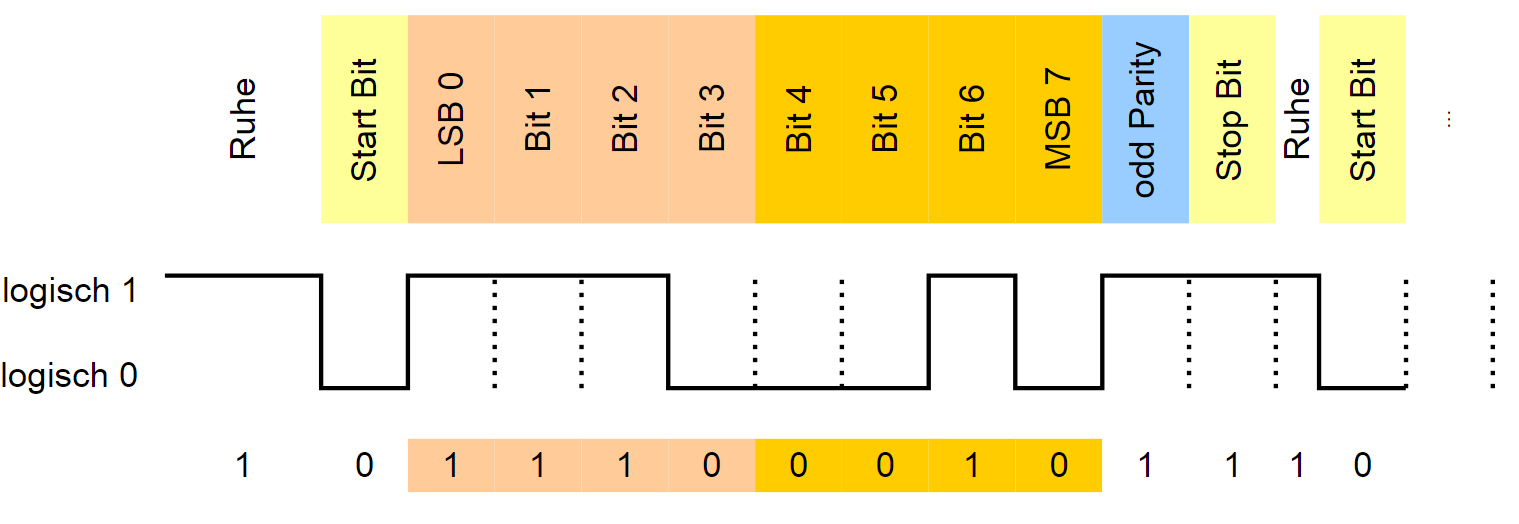
\includegraphics[width=0.90\textwidth]{bilder/uart}
	\caption{Signalübertragung über das UART-Protokoll}
	\label{fig:uart}
\end{figure}

Die Daten werden zu Paketen von meist 8 Bit (entspricht 1 Byte), wobei die Sende-Reihenfolge in der Regel vom \textit{least significant bit} (LSB) zum \textit{most significant bit} versendet wird (vgl. Abb. \ref{fig:uart}). Wenn bei einer UART-Verbindung gerade keine Daten übertragen werden, liegt eine ``high''-Spannung an (logisch ``1''). Die Übertragung beginnt mit einem Start-Bit (logisch ``0'') für einen UART-Taktzyklus, wonach die Datenbits folgen. Je nach Implementierung kann eine Parität\footnote{Binäre Angabe, ob das Datenpaket eine gerade oder ungerade Anzahl ``Einsen'' enthält.} folgen oder weggelassen werden. Ein Stop-Bit beendet die Transmission eines Datenpaketes. \\

Ein \textit{UART-Taktzyklus} beschreibt, wie lange die Spannung eines einzelnen Symbols anliegt. Die entsprechende Einheit wird in \textit{Baud} angegeben und entspricht $1 * s^{-1}$. Bei einer Übertragungsrate von 9600 Baud liegt ein Bit also für $1 / 9600s = 104,167 \mu s$ am Ausgang Tx an. \\


%!TEX root = ../ecdsa.tex

\chapter{Implementierung} \label{sec:impl}

%%%%%%%%%%%%%%%%%%%%%%%%%%%%%%%%%%%%%%%%%%%%%%%%%%%%%%%%%%%%%
\section{Architektur \& Moduldesign} 
\label{sec:march}
Die Architektur der VHDL-Implementierung verwendet einen modularen Ansatz. Die zentrale Komponente wird durch den Controller repräsentiert, der den Zustandsautomat, die ECC-, sowie die arithmetischen Operationen beinhaltet und damit die ECDSA-Funktionen (Signieren, Verifizieren)  implementiert. Abbildung \ref{fig:vhdl-impl-arch} zeigt den grundlegenden Aufbau des Systems.   

\begin{figure}[H]
	\centering
  	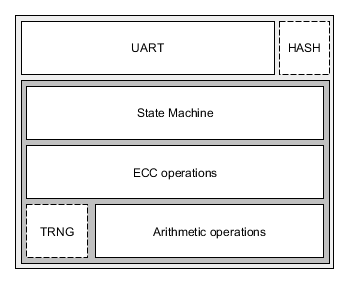
\includegraphics[width=0.7\textwidth]{bilder/vhdl_overview.png}
	\caption{Modulübersicht der FPGA-Hardware}
	\label{fig:vhdl-impl-arch}
\end{figure}
 
Die Umschaltung zwischen den verschiedenen Algorithmen findet über einen Zustandsautomat (engl. State Machine) statt. Die Hardware-Implementierung kann zwischen den Modi Signieren und Verifizieren unterschieden. Die Umschaltung findet über die UART-Schnittstelle statt, indem der Datenstrom analysiert wird. Eine detaillierte Beschreibung ist in Abschnitt \ref{sec:uartimpl} zu finden. Je nach gewünschter Funktion, werden andere Parameter über UART empfangen bzw. zurückgeschickt. Eine Übersicht der Parameter beinhaltet Tabelle \ref{tab:vhdl-impl-uart-data}. \\

\begin{table} [h]
	\centering 
	\begin{tabular}{ | p{3cm} | p{2cm} | p{6cm} | }
		\hline
		\textbf{Funktion} & \textbf{Typ} & \textbf{Parameter} \\
		\hline
		Signieren & Input &  Nachricht $m$ (163 Bit) \\
		\hline
		Signieren & Ouput & Signatur $(r,s)$ (326 Bit) \\
		\hline
		Verifizieren & Input & Nachricht $m$ (163 Bit) \\
		\hline
		Verifizieren & Input & Signatur $(r,s)$ (326 Bit) \\
		\hline
		Verifizieren & Output & Ergebnis der Verifizierung (1 Bit) \\
		\hline
	\end{tabular}
	\caption{Eingabe- und Ausgabedaten der VHDL-Implementierung}
	\label{tab:vhdl-impl-uart-data}
\end{table}
 
Wie bereits in Kapitel \ref{sec:planung} erwähnt, wurde auf eine sicherheitsorientierte Implementierung des Algorithmus verzichtet, sodass anstatt eines ``echten'' Zufallszahlengenerators  (engl. True Random Number Generator, TRNG), lediglich eine festgelegte Konstante zum Einsatz kommt. Hauptgrund für diese Entscheidung begründet sich mit der fehlenden Hardware zum Generieren einer sicheren Zufallszahl. Als eine weitere Vereinfachung wurde auf eine Einheit zum Generieren eines Hashes verzichtet, um den Fokus auf die Implementierung der ECC-Operationen zu lenken, ohne die Messergebnisse durch die HASH-Generierung zu verfälschen. Aus Gründen der Vollständigkeit sind beide Komponenten dennoch in Abbildung \ref{fig:vhdl-impl-arch} zu finden. 

%%%%%%%%%%%%%%%%%%%%%%%%%%%%%%%%%%%%%%%%%%%%%%%%%%%%%%%%%%%%%

\section{Parameter}
\label{vhdl-impl-parameter}

Die gesamte VHDL-Implementierung setzt ausschließlich auf VHDL-typische \texttt{Generics}. Diese werden über das globale Paket \texttt{tld\_ecdsa\_package} verwaltet. Neben den Parametern enthält das Paket globale Hilfsfunktionen, die zum Beispiel eine Matrix-Reduktion durchführen. Tabelle \ref{tab:vhdl-impl-param} zeigt eine Übersicht der wichtigsten Parameter.
\\ \\
Wie der Tabelle \ref{tab:vhdl-impl-param} zu entnehmen ist, sind in der Datei auch der private, der öffentliche Schlüssel und die k-Konstante  zu finden. Die Schlüssel wurden direkt als Konstanten hinterlegt, um die Kommunikation über die UART-Schnittstelle zu vereinfachen. Für den Einsatz der Software in einer produktiven Umgebung sollte  der öffentliche Schlüssel austauschbar sein, sodass auch Signaturen von Anderen verifiziert werden können. Das gleiche gilt für den privaten Schlüssel, um in der Lage zu sein, nachträglich die Schlüssel aus sicherheitsgründen auszutauschen oder allgemein Signaturen mit verschiedenen Schlüsseln zu erstellen.
\\ \\
Durch den Einsatz der generischen Implementierung ist es möglich, Parameter nachträglich zu ändern, um beispielsweise eine andere Schlüssellänge oder Kurvenparameter zu verwenden. Ein Nachteil dagegen ist, dass durch die generische Implementierung weniger Spielraum für Performanz-Optimierungen besteht. Da mit wachsender Leistungsfähigkeit heutiger Systeme aber auch die Anforderung an kryptografische steigt, wurde die nachträgliche Anpassbarkeit der Parameter als wichtiger angesehen. \\

\begin{table} [h]
	\centering 
	\begin{tabular}{ | p{3cm} | p{12cm} | }
		\hline
		\textbf{Parameter} & \textbf{Beschreibung}\\
		\hline
		M & Bitbreite des Schlüssels bzw. der Daten (z.B. 163) \\
		\hline
		N & Modolo-Parameter der Kurve (Bestandteil des ECDSA-Algorithmus) \\
		\hline
		A & A-Parameter der Kurve (Bestandteil des ECDSA-Algorithmus) \\
		\hline
		P & Anzahl der Elemente im GF($2^M$) \\
		\hline
		xG & x-Komponenten des Generator-Punktes \\
		\hline
		yG & y-Komponenten des Generator-Punktes \\
		\hline
		dA & Privater Schlüssel für die Signierung \\
		\hline
		xQ & x-Komponenten des öffentlichen Schlüssel für die Verifizierung \\
		\hline
		yQ & y-Komponenten des öffentlichen Schlüssel für die Verifizierung \\
		\hline
		k & (statische) Zufallszahl \\
		\hline
		BAUD\_RATE & Eingestellte Baud-Rate der UART-Schnittstelle \\
		\hline
	\end{tabular}
	\caption{Parameter der VHDL-Implementierung}
	\label{tab:vhdl-impl-param}
\end{table}


%%%%%%%%%%%%%%%%%%%%%%%%%%%%%%%%%%%%%%%%%%%%%%%%%%%%%%%%%%%%%

\section{Top-Level-Entität}
\label{vhdl-impl-tld}

Wie bereits erwähnt kommuniziert die Top-Level-Entität über eine serielle RS232-Schnittstelle mit einem Computer, um Daten auszutauschen. Dazu werden lediglich zwei Pins zur UART-Kommunikation, sowie ein globales 50Mhz-Takt- und ein Resetsignal benötigt. Tabelle \ref{tab:vhdl-impl-tld-ecdsa-param} beschreibt die Parameter der Entität \\

\begin{figure}[thb]
	\centering
	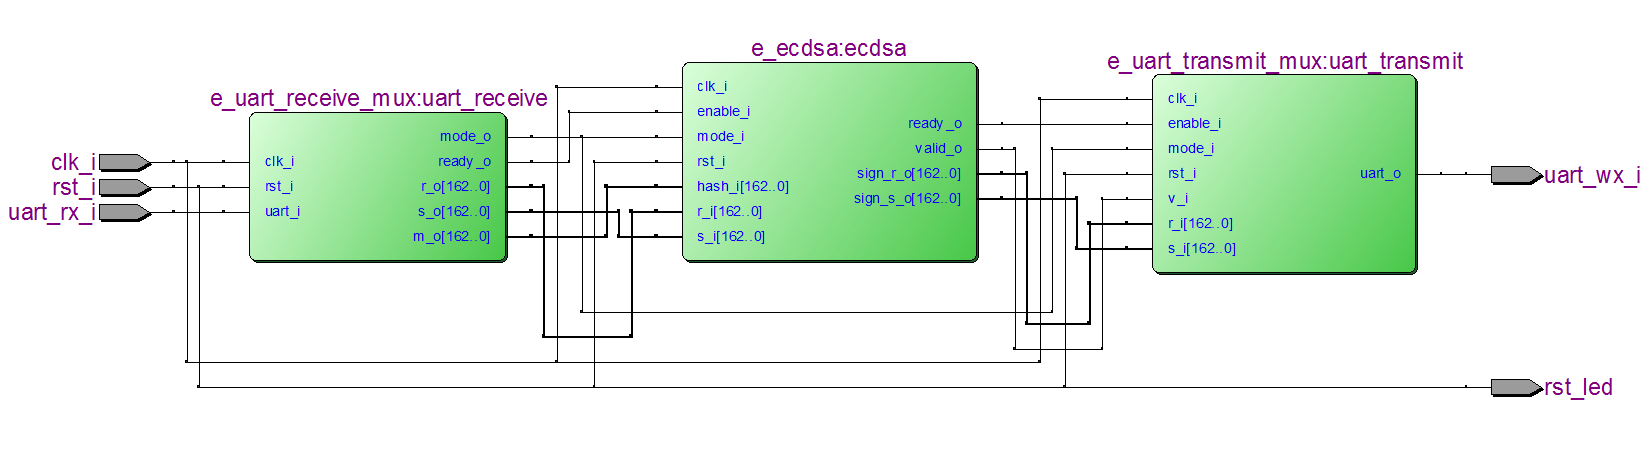
\includegraphics[width=\textwidth]{bilder/tle}
	\caption{Top-Level-Entity der VHDL-Implementierung}
	\label{fig:vhdl-impl-tle}
\end{figure}

Nach vollständigem Erhalt der Daten, die sich je nach Algorithmus unterscheiden (vgl. Tabelle \ref{tab:vhdl-impl-uart-data}), werden diese dem zentralen Modul \texttt{e\_ecdsa} bereitgestellt. Über binäre Eingänge wird festgelegt, welcher Modus (Signieren vs. Verifizieren, Pin \texttt{mode\_i}) verwendet und wann die Berechnung gestartet werden soll (Pin \texttt{enable\_i}). Sobald die ECDSA-Entität die Berechnung abgeschlossen hat, wird ein binäres Flag gesetzt, sodass die Daten über das Modul \texttt{e\_uart\_transmit\_mux} zurückschickt werden können. \\
 
\begin{table} [h]
	\centering 
	\begin{tabular}{ | p{3cm} | p{12cm} | }
		\hline
		\textbf{Parameter} & \textbf{Beschreibung}\\
		\hline
		clk\_i & Globales Taktsignal \\
		\hline
		rst\_i & Resetsignal \\
		\hline
		uart\_rx\_i & Pin zum Lesen der UART-Kommunikation \\
		\hline
		uart\_tx\_i & Pin zum Schreiben der UART-Kommunikation \\
		\hline
		rst\_led & LED zur Kennzeichnung ob das Reset-Signal aktiv ist \\
		\hline
	\end{tabular}
	\caption{Eingabe- und Ausgabeparameter der Haupt-Entität}
	\label{tab:vhdl-impl-tld-ecdsa-param}
\end{table} 


%%%%%%%%%%%%%%%%%%%%%%%%%%%%%%%%%%%%%%%%%%%%%%%%%%%%%%%%%%%%%
\section{ECDSA-Implementierung}
\label{vhdl-impl-general}

\subsection{Allgemeiner Aufbau der VHDL-Entitäten}
\label{vhdl-impl-general-entity}

Jede Entität, sei es eine mathematische oder eine zusammengesetzte Komponente wie die ECC-Operationen, verwendet den selben Aufbau. So besitzen die Entitäten neben einem globalen Takt- und Resetsignal ein Aktivierungs- und ein Status-Flag, sowie eine beliebige Anzahl anwendungsabhängiger Eingabe- bzw. Ausgabeparameter. Eine Übersicht der Parameter ist in Tabelle \ref{tab:vhdl-impl-ecdsa-general} zu finden. \\

\begin{table} [h]
	\centering 
	\begin{tabular}{ | p{3cm} | p{12cm} | }
		\hline
		\textbf{Parameter} & \textbf{Beschreibung}\\
		\hline
		clk\_i & Globales Taktsignal \\
		\hline
		rst\_i & Resetsignal \\
		\hline
		enable\_i & Flag zum Aktivieren der Berechnung \\
		\hline
		x\_n\_i & Eingabeparameter 1-n \\
		\hline
		z\_m\_o & Ausgabeparameter 1-m \\
		\hline
		p\_q\_i & Zusatzparameter 1-q \\
		\hline
		ready\_o & Flag welches anzeigt, ob die Berechnung abgeschlossen ist \\
		\hline
	\end{tabular}
	\caption{Allgemeine Eingabe- und Ausgabeparameter der Entitäten}
	\label{tab:vhdl-impl-ecdsa-general}
\end{table}

Das Aktivierungs-Flag startet unmittelbar bei einem ``High''-Pegel die Berechnung. Bleibt das Signal aktiviert, nachdem die Berechnung abgeschlossen ist, wird eine erneute Berechnung gestartet. Das Status-Flag führt standardmäßig einen ``High''-Pegel, der auf ``Low'' wechselt, sobald das Aktivierungs-Flag gesetzt wurde. Ist die Berechnung abgeschlossen ist, wird das Status-Flag wieder auf ``High'' gesetzt.
\\ \\
Die Ablaufsteuerung findet über einen Zustandsautomaten statt. Die grundlegende Struktur der Automaten zeigt Listing \ref{lst-fsm}\\ 

\begin{lstlisting}[language=Python,frame=single,label=lst-fsm,caption=Grundstruktur der Zustandsautomaten]
CASE current_state IS
  WHEN 0 TO 1 => enable_fct_i <= '0'; ready_o <= '1';;
  WHEN 2 => enablefct_i <= '1'; ready_o <= '0';
  ...
  WHEN N => enable_fct_i <= '0'; ready_o <= '0';
END CASE;

IF rst_i = '1' THEN
  current_state <= 0;
ELSIF clk_i'event and clk_i = '1' THEN
  CASE current_state IS
    WHEN 0 => 
      IF enable_i = '0' THEN 
        current_state <= 1; 
      END IF;
    WHEN 1 => 
      IF enable_i = '1' THEN 
        current_state <= 2; 
      END IF;
    WHEN 2 => current_state <= 3;
    ...
    WHEN N => current_state <= 0; 
  END CASE;
END IF;
\end{lstlisting}

\subsection{ECDSA-Algorithmus}

Die Implementierung des ECDSA-Algorithmus findet über die Entität \texttt{e\_ecdsa} statt. Für die Umschaltung zwischen Signieren und Verfifizieren wird ein Zustandsautomat verwendet, der im wesentlichen im Abhängigkeit des Parameters \texttt{mode\_i} zwischen den Algorithmen wechselt. Damit kann pro Ablauf immer nur ein Algorithmus zur Zeit gestartet werden.
\\ \\
Die Implementierung der Algorithmen folgt dem Ablauf aus Kapitel \ref{ecdsa-algo}. Der Ablauf ist streng sequentiell, wobei versucht wird, einen maximalen Parallelisierungsgrad anzustreben. So werden beispielsweise bei der Verifikation die Variablen $u_1$ und $u_2$ parallel berechnet. Abbildung \ref{fig:vhdl-impl-ecdsa} verdeutlicht den Ablauf.

\begin{figure}[thb]
	\centering
	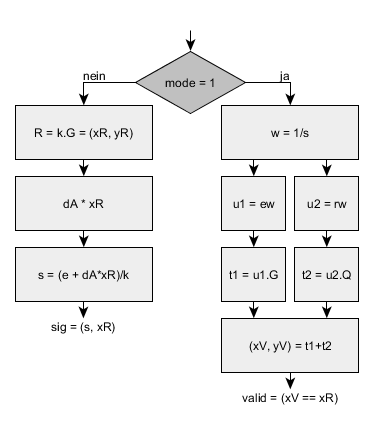
\includegraphics[width=0.6\textwidth]{bilder/vhdl_ecdsa.png}
	\caption{Vereinfachter Ablauf des ECDSA-Algorithmus}
	\label{fig:vhdl-impl-ecdsa}
\end{figure}

Die Algorithmen sind so umgesetzt, dass jede Operation über eine eigene Entität abgebildet wird. So besteht das Signieren aus 3 Entitäten (1x Punktmultiplikation, 1x Multiplizierer, 1x Dividierer), während die Verifikation aus 6 Entitäten (1x Punktaddition, 2x Punktmultiplikation, 2x Multiplizierer, 1xInverter) besteht. Grund für die Verdopplung liegt in erster Linie an der deutlich einfacheren und übersichtlicheren Implementierung. Der Nachteil dagegen ist, dass der Ressourcenverbrauch deutlich höher ist. Da die eingesetzte Hardware aber genügend Ressourcen zur Verfügung stellt, wurde auf eine Optimierung verzichtet. Ein weiterer Vorteil dieser Implementierung ist, dass theoretisch parallel signiert und verifiziert werden kann, was bei einer gemeinsamen Nutzung von Entitäten aufgrund der Umschaltlogik nicht möglich wäre. Für die zeitliche Aktivierung der Entitäten wird wieder auf den Zustandsautomat zurückgegriffen, der die in Abschnitt \ref{vhdl-impl-general-entity} erwähnten Aktivierungs- bzw. Status-Flags verwendet.
\\ \\
Abschließend sei erwähnt, dass der implementierte Algorithmus kleinere Teilkomponenten der Originalfassung nicht berücksichtigt. So wird auf die Überprüfung von Zwischenergebnissen verzichtet. Grund hierfür liegt im wesentlichen an der Tatsache, dass eine ungünstige Wahl der Zufallszahl zu Fehlern führen kann. Da diese Implementierung eine günstige Konstante verwendet, wurde auf ein Abfragen verzichtet. Durch die gewählte Struktur lassen sich  solche Abfragen aber mit wenig Aufwand einbauen, da lediglich der Zustandsautomat angepasst werden muss. Das gleiche gilt für ein nachträgliches Hinzufügen der Zufallszahlgenerierung. \\

\begin{table} [h]
	\centering 
	\begin{tabular}{ | p{3cm} | p{12cm} | }
		\hline
		\textbf{Parameter} & \textbf{Beschreibung}\\
		\hline
		clk\_i & Globales Taktsignal \\
		\hline
		rst\_i & Resetsignal \\
		\hline
		enable\_i & Flag zum Aktivieren der Berechnung \\
		\hline
		mode\_i & Flag zum Umschalten zwischen Signieren und Verifizieren \\
		\hline
		hash\_i & Eingabe Text \\
		\hline
		r\_i & R-Komponente der zu verifizierenden Signatur \\
		\hline
		s\_i & S-Komponente der zu verifizierenden Signatur \\
		\hline
		ready\_o & Status-Flag ob die Berechnung abgeschlossen ist  \\
		\hline
		valid\_o & Flag ob die zu verifizierenden Signatur valide ist \\
		\hline
		r\_o & R-Komponente der erstellten Signatur \\
		\hline
		s\_s & S-Komponente der erstellten Signatur \\
		\hline
	\end{tabular}
	\caption{Eingabe- und Ausgabeparameter der ECDSA-Entität}
	\label{tab:vhdl-impl-ecdsa-param}
\end{table}

\subsection{Punktaddition und -dopplung}
Die Punktaddition und Punktdopplung basieren auf den Formeln aus Abschnitt \ref{sec:ell}. \\

\begin{table} [h]
	\centering 
	\begin{tabular}{ | p{3cm} | p{12cm} | }
		\hline
		\textbf{Parameter} & \textbf{Beschreibung}\\
		\hline
		clk\_i & Globales Taktsignal \\
		\hline
		rst\_i & Resetsignal \\
		\hline
		enable\_i & Flag zum Aktivieren der Berechnung \\
		\hline
		x1\_i & x Komponente des Basis-Punktes \\
		\hline
		y1\_i & y Komponente des Basis-Punktes \\
		\hline
		x2\_o & x Komponenten der Punktdopplung \\
		\hline
		y2\_o & y Komponenten der Punktdopplung \\
		\hline
		ready\_o & Status-Flag ob die Berechnung abgeschlossen ist  \\
		\hline
		\hline
	\end{tabular}
	\caption{Eingabe- und Ausgabeparameter der Punktdopplungs-Entität}
	\label{tab:vhdl-impl-eccdouble-param}
\end{table}

Der zugrundeliegende Ablauf ist identisch mit der Implementierung des ECDSA-Algorithmus, wobei sich lediglich die Formeln unterscheiden. So wird für jede mathematische Operation eine separate VHDL Entität verwendet, die sequentiell über die Aktivierungs- bzw. Status-Flags abgearbeitet werden. Die Umschaltung findet wieder über einen Zustandsautomat statt.

\begin{figure}[thb]
	\centering
	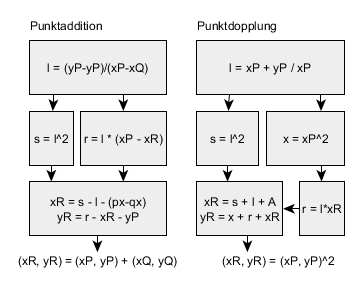
\includegraphics[width=0.7\textwidth]{bilder/vhdl_pa_pd.png}
	\caption{Vereinfachter Ablauf des Punktaddition und -dopplung}
	\label{fig:vhdl-impl-pa-pd}
\end{figure}

Abbildung \ref{fig:vhdl-impl-pa-pd} zeigt den vereinfachten Ablauf der Berechnung. Wie bereits beim ECDSA-Algorithmus wird auch hier ein maximaler Parallelisierungsgrad angestrebt. \\

\begin{table} [h]
	\centering 
	\begin{tabular}{ | p{3cm} | p{12cm} | }
		\hline
		\textbf{Parameter} & \textbf{Beschreibung}\\
		\hline
		clk\_i & Globales Taktsignal \\
		\hline
		rst\_i & Resetsignal \\
		\hline
		enable\_i & Flag zum Aktivieren der Berechnung \\
		\hline
		x1\_i & x Komponente des ersten Punktes \\
		\hline
		y1\_i & y Komponente des ersten Punktes \\
		\hline
		x2\_i & x Komponente des zweiten Punktes \\
		\hline
		y2\_i & y Komponente des zweiten Punktes \\
		\hline
		x3\_o & x Komponenten des Additionsergebnisses \\
		\hline
		y3\_o & y Komponenten des Additionsergebnisses \\
		\hline
		ready\_o & Status-Flag ob die Berechnung abgeschlossen ist  \\
		\hline
		\hline
	\end{tabular}
	\caption{Eingabe- und Ausgabeparameter der Punktadditions-Entität}
	\label{tab:vhdl-impl-eccadd-param}
\end{table}

\subsection{Punktmultiplikation}
Die Punktmultiplikation basiert auf dem Double-And-Add-Algorithmus, der die Zeit für die Berechnung deutlich verkürzt. Der Pseudocode ist in Listing \ref{lst-pm-algo} zu finden.  \\

\begin{lstlisting}[language=Python,frame=single,label=lst-pm-algo,caption=Pseudocode des Double-And-Add Algorithmus]
N = P; Q = 0

for i from 0 to m do
  if di = 1 then
    Q = point_add(Q, N)
  N = point_double(N)

return Q
\end{lstlisting}

Würde anstatt des Double-And-Add-Algorithmus der triviale Algorithmus verwendet werden, so würden für $m = 100 P$ $100$ Punktadditionen benötigt werden, um das Ergebnis zu erhalten. Durch den Einsatz des Double-And-Add-Algorithmus lässt sich die Gleichung umschreiben als $m = 2(2[P + 2(2[2(P + 2P)])])$. Dadurch werden lediglich 6 Punktdopplungen und nur noch 2 Punktadditionen benötigt. \\

\begin{table} [h]
	\centering 
	\begin{tabular}{ | p{3cm} | p{12cm} | }
		\hline
		\textbf{Parameter} & \textbf{Beschreibung}\\
		\hline
		clk\_i & Globales Taktsignal \\
		\hline
		rst\_i & Resetsignal \\
		\hline
		enable\_i & Flag zum Aktivieren der Berechnung \\
		\hline
		xp\_i & x Komponente des Basis-Punktes \\
		\hline
		yp\_i & y Komponente des Basis-Punktes \\
		\hline
		k\_i & Multiplikations-Faktor \\
		\hline
		xq\_o & x Komponenten des Ergebnis-Punktes \\
		\hline
		yq\_o & y Komponenten des Ergebnis-Punktes \\
		\hline
		ready\_o & Status-Flag ob die Berechnung abgeschlossen ist  \\
		\hline
		\hline
	\end{tabular}
	\caption{Eingabe- und Ausgabeparameter der Punktmultiplikations-Entität}
	\label{tab:vhdl-impl-eccmul-param}
\end{table}

\subsection{Polynomreduktion}
Berechnungen wie die Multiplikation führen zu einem Polynom mit einen Grad von $2m-2$, sodass eine Reduktion auf eine Breite von $m$ durchgeführt werden muss.
\\ \\
Für die Reduktion wird eine allgemeine Variante eingesetzt, die eine Nachschlagetabelle anhand des Modulo-Wertes erstellt. Anhand dieser Tabelle wird anschließend ein Eingangspolynom durch Bitverschiebungen, Bitprüfungen und Additionen reduziert.

\subsection{Multiplizierer und Dividierer}
Die Multiplizierer-Entität basiert auf einer klassischen Polynom-Multiplikation, die eine Reihe von Bitverschiebungen, XOR-Verknüpfungen und Polynomreduktionen verwendet. \\

\begin{table} [h]
	\centering 
	\begin{tabular}{ | p{3cm} | p{12cm} | }
		\hline
		\textbf{Parameter} & \textbf{Beschreibung}\\
		\hline
		clk\_i & Globales Taktsignal \\
		\hline
		rst\_i & Resetsignal \\
		\hline
		enable\_i & Flag zum Aktivieren der Berechnung \\
		\hline
		a\_i & Eingabewert 1 \\
		\hline
		b\_i & Eingabewert 2 \\
		\hline
		z\_o & $z = a*b \mod p$ in $GF(2^M)$ \\
		\hline
		ready\_o & Status-Flag ob die Berechnung abgeschlossen ist  \\
		\hline
		\hline
	\end{tabular}
	\caption{Eingabe- und Ausgabeparameter der Multiplizierer-Entität}
	\label{tab:vhdl-impl-mult-param}
\end{table}

Für den Dividierer wurden zwei verschiedenen Implementierungen verwendet, um Laufzeitunterschiede zu messen. Die erste Variante basiert auf einer klassischen Polynomdivision, während die zweite Implementierung eine Multiplikation mit dem Inversen durchführt. \\

\begin{table} [h]
	\centering 
	\begin{tabular}{ | p{3cm} | p{12cm} | }
		\hline
		\textbf{Parameter} & \textbf{Beschreibung}\\
		\hline
		clk\_i & Globales Taktsignal \\
		\hline
		rst\_i & Resetsignal \\
		\hline
		enable\_i & Flag zum Aktivieren der Berechnung \\
		\hline
		g\_i & Eingabewert 1 \\
		\hline
		h\_i & Eingabewert 2 \\
		\hline
		z\_o & $z = g/h \mod p$ in $GF(2^M)$ \\
		\hline
		ready\_o & Status-Flag ob die Berechnung abgeschlossen ist  \\
		\hline
		\hline
	\end{tabular}
	\caption{Eingabe- und Ausgabeparameter der Dividierer-Entität}
	\label{tab:vhdl-impl-divider-param}
\end{table}

\subsection{Quadrier}
Der Quadrierer verwendet eine optimierte Implementierung für Polynome, sodass keine klassische Multiplikation verwendet werden muss. Nach der Bestimmung des Qadradats findet anschließend eine Polynomreduktion statt. 

\begin{table} [h]
	\centering 
	\begin{tabular}{ | p{3cm} | p{12cm} | }
		\hline
		\textbf{Parameter} & \textbf{Beschreibung}\\
		\hline
		clk\_i & Globales Taktsignal \\
		\hline
		rst\_i & Resetsignal \\
		\hline
		enable\_i & Flag zum Aktivieren der Berechnung \\
		\hline
		d\_i & Eingabewert, von welchem das Quadrat gebildet wird \\
		\hline
		c\_o & $c = d^2 \mod p$ in $GF(2^M)$ \\
		\hline
		ready\_o & Status-Flag ob die Berechnung abgeschlossen ist  \\
		\hline
		\hline
	\end{tabular}
	\caption{Eingabe- und Ausgabeparameter der Quadrierer-Entität}
	\label{tab:vhdl-impl-squarer-param}
\end{table}

\subsection{Inverter}
Zum Bestimmen des Inversen wird der erweiterte euklidische Algorithmus eingesetzt. Der Algorithmus bedient sich der Tatsache, dass wenn der Algorithmus das Tripel $d = ggt(a, b), s, t$ ermittelt, ist entweder $d=1$ und damit $1 = t*b \mod a$, sodass $t$ das multiplikative Inverse von $b \mod a$ ist, oder es gilt $d \neq 1$, was bedeutet, dass $b \mod a$ kein Inverses hat. \\

\begin{table} [h]
	\centering 
	\begin{tabular}{ | p{3cm} | p{12cm} | }
		\hline
		\textbf{Parameter} & \textbf{Beschreibung}\\
		\hline
		clk\_i & Globales Taktsignal \\
		\hline
		rst\_i & Resetsignal \\
		\hline
		enable\_i & Flag zum Aktivieren der Berechnung \\
		\hline
		a\_i & Eingabewert, von welchem das Inverse gebildet wird \\
		\hline
		z\_o & $z = 1/x \mod p$ in $GF(2^M)$ \\
		\hline
		ready\_o & Status-Flag ob die Berechnung abgeschlossen ist  \\
		\hline
		\hline
	\end{tabular}
	\caption{Eingabe- und Ausgabeparameter der Inverter-Entität}
	\label{tab:vhdl-impl-inverter-param}
\end{table}

\subsection{Addierer / Subtrahierer}
Die Addition bzw. Subtraktion ist im $GF(2^M)$ trivial, da $-1 = 1$ gilt. Somit muss lediglich eine XOR-Verknüpfung der Operanden durchgeführt werden .  Aufgrund der Einfachheit wurde auf eine separate Entität verzichtet.

\subsection{Test- und Verifizierung}
Für den Test- und die Verifizierung der Entities werden zwei verschiedene Arten von Testbenches verwendet. Die triviale Variante dient lediglich dem kurzen Funktionstest der Entität. Dazu werden lediglich einige statische Werte und Randbedingungen abgefragt, um die Entwicklung der Entitäten zu unterstützen. Die ``echten'' Testbenches dagegen versuchen anhand dynamisch generierter Testdaten die Kombination verschiedener Entitäten zu verifizieren.
\\ \\
Der Tabelle \ref{tab:vhdl-impl-testbenches} ist zu entnehmen, dass beispielsweise die Punktmultiplikation neben der eigentlichen Multiplikation auch die Punktaddition und damit auch die dafür notwendigen mathematischen Grundoperatoren verifiziert. Da es die Testbench erfordert, dass verschiedene Entitäten separat entwickelt werden, was im Fehlerfall die Identifizierung deutlich erschwert, wurden weitere einfachere Testbenches geschrieben, um zunächst die Basisfunktionalität der Entitäten zu verifizieren.
\\ \\
Neben dem reinen Überprüfen der Bedingungen wird teilweise zusätzlich überprüft, ob die Berechnung in einer definierten Anzahl von Taktzyklen abgeschlossen wurde.

\begin{table} [h]
	\centering 
	\begin{tabular}{ | p{5cm} | p{2cm} | p{8cm} | }
		\hline
		\textbf{Beschreibung} & \textbf{Typ} & \textbf{Bedingung}\\
		\hline
		tb\_ecdsa &  dynamisch & \parbox[t]{5cm}{$(r,s)=sign(m)$\\$verify((r,s),m)=True$}  \\
		\hline
		tb\_gf2m\_multiplier & statisch & $a * b = CONST$ \\
		\hline
		tb\_gf2m\_squarer & statisch & $ a * a = CONST$ \\
		\hline
		tb\_gf2m\_eea\_inversion & dynamisch & $x * x^-1 = 1$ \\
		\hline
		tb\_gf2m\_divider & dynamisch & \parbox[t]{5cm}{$c=a/b$\\$c*b=a$} \\
		\hline
		tb\_gf2m\_point\_addition & statisch & $P+Q = CONST $ \\
		\hline
		tb\_gf2m\_point\_doubling & statisch & $P+P = CONST$ \\
		\hline
		tb\_gf2m\_point\_multiplication & dynamisch & \parbox[t]{10cm}{$k.P = (k-1).P + P$\\$k.P = (n-1).P = -P = (xP, xP+yP)$} \\
		\hline
	\end{tabular}
	\caption{Beschreibung der Testbenches}
	\label{tab:vhdl-impl-testbenches}
\end{table}

%%%%%%%%%%%%%%%%%%%%%%%%%%%%%%%%%%%%%%%%%%%%%%%%%%%%%%%%%%%%%
\section{Kommunikation der UART-Verbindung} \label{sec:uartimpl}

Die UART-Komponenten übernehmen wie in Kap. \ref{sec:iuart} beschrieben neben der externen Kommunikation auch die Transformation der Daten. Dabei wird der Rx-Input\footnote{Das Rx-Signal wird erst nach Einsynchronisation mit zwei aufeinanderfolgenden Flip-Flops verarbeitet.} nach dem Empfangen über Register mit einem Parallel-Ausgang zur Verfügung gestellt. Abbildung \ref{fig:uartrx} zeigt die Verschaltung des \textbf{Receivers} mit den Schieberegistern im RTL Viewer der Entwicklungsumgebung. \\

\begin{figure}[thb]
	\centering
  	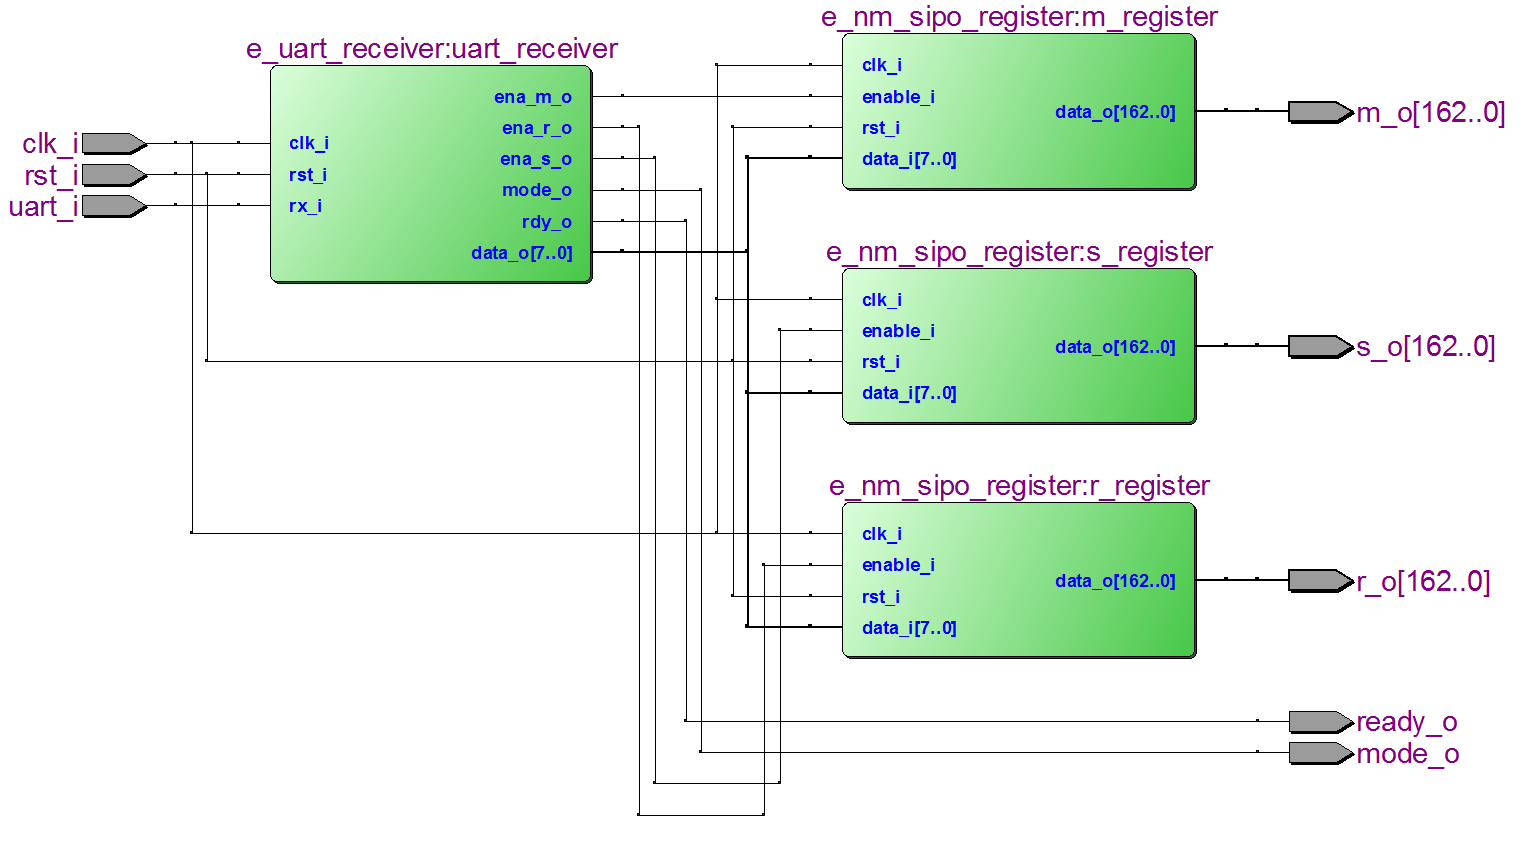
\includegraphics[width=0.9\textwidth]{bilder/uart-receiver}
	\caption{Ansicht des UART-Receivers im RTL Viewer}
	\label{fig:uartrx}
\end{figure}

Der Receiver selbst enthält einen Zustandsautomaten, der den Eingabedatenstrom in die zwei Modi \texttt{Signieren} und \texttt{Verifizieren} klassifiziert. Anhand der Zustände werden die Steuerungssignale am Modulausgang (\textit{enable}-Signale für die Punkte $r$ und $s$ auf der elliptischen Kurve sowie die Nachricht) so geschaltet, sodass jeweils die entsprechenden Eingabewörter in den dafür vorgesehenen Registern landen\footnote{phase1 = $r$, phase2 = $s$, phase3 = $message$} (vgl. Abb. \ref{fig:uart-receiver-phase}. Hierfür gibt es zwei vorangegangene Phase, in denen der Modus durch das erste empfangene Byte bestimmt wird (\textit{dmode}) und anschließend über die Dauer eines Taktzyklus umgeschaltet wird (\textit{smode}). \\

\begin{figure}[thb]
	\centering
  	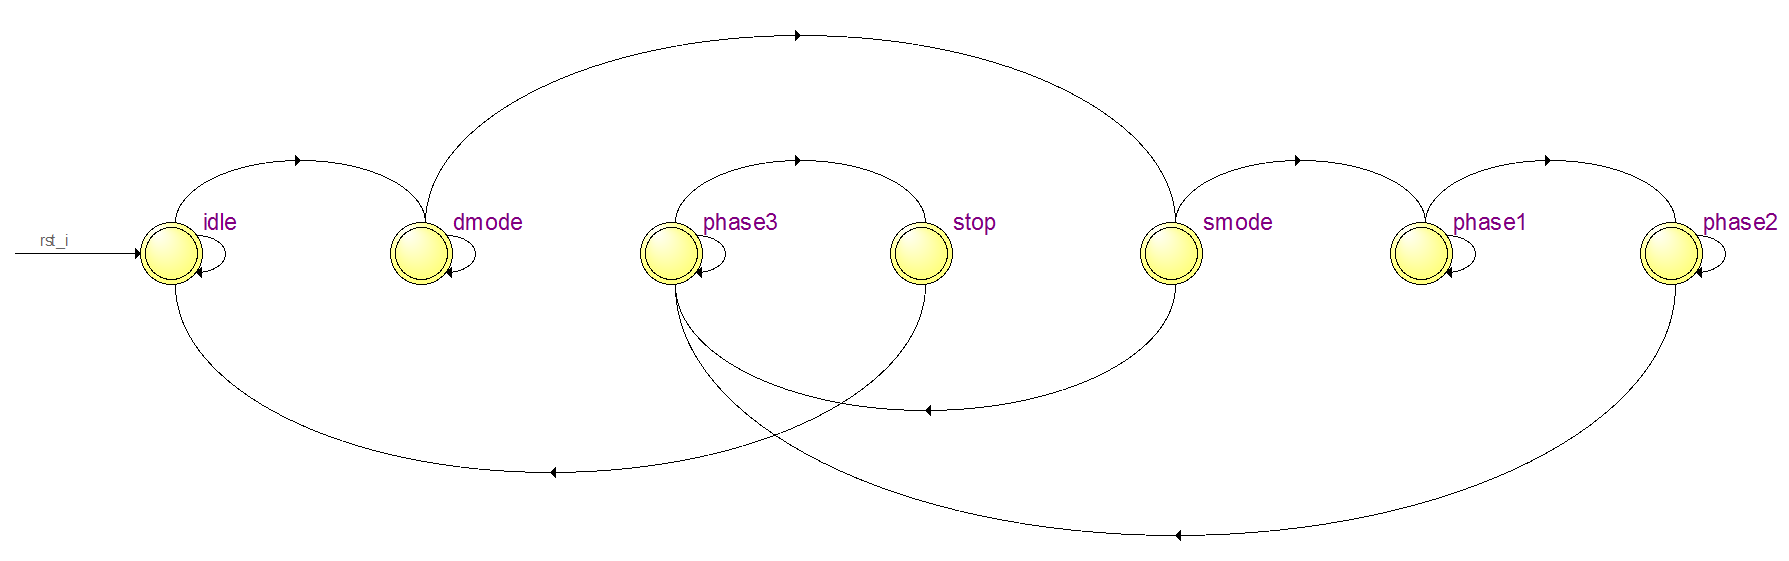
\includegraphics[width=\textwidth]{bilder/uart-receiver-phase}
	\caption{Zustandsautomat des Receivers zu Phasen-Bestimmung beim Empfang}
	\label{fig:uart-receiver-phase}
\end{figure}

Die Phasen des gezeigten Automaten bilden eine Abstraktionsebene über der eigentlichen Erkennung der sequentiellen Datenbits am Rx-Eingang. Ein weiterer Zustandsautomat (s. Anhang \ref{fig:uart-receiver-data}) agiert innerhalb eines UART-Datenpaketes (Start-Bit, 8 Bit Daten, Stop-Bit) und speichert ein einzelnes Byte zwischen zur Weiterverarbeitung. Der erste Byte für den Modus muss dabei entweder ``00000000b'' für das Signieren oder ``11111111b'' für das Verifizieren sein. Der Modus wird als binäres Signal für nachfolgende Module nach außen geführt. \\

Der \textbf{UART-Transmitter} beinhaltet zwei Schieberegister, die einen parallelen Eingang mit einem Byte-weise seriellen Ausgang besitzen (vgl. Abb. \ref{fig:uarttx}). Das \texttt{e\_uart\_transmit}-Modul steuert diese Register über einen internen Zustandsautomaten gibt die entsprechenden Steuerungssignale nach außen an die beiden Multiplexer, welche die \textit{enable}-Eingänge anspricht. \\

\begin{figure}[H]
	\centering
  	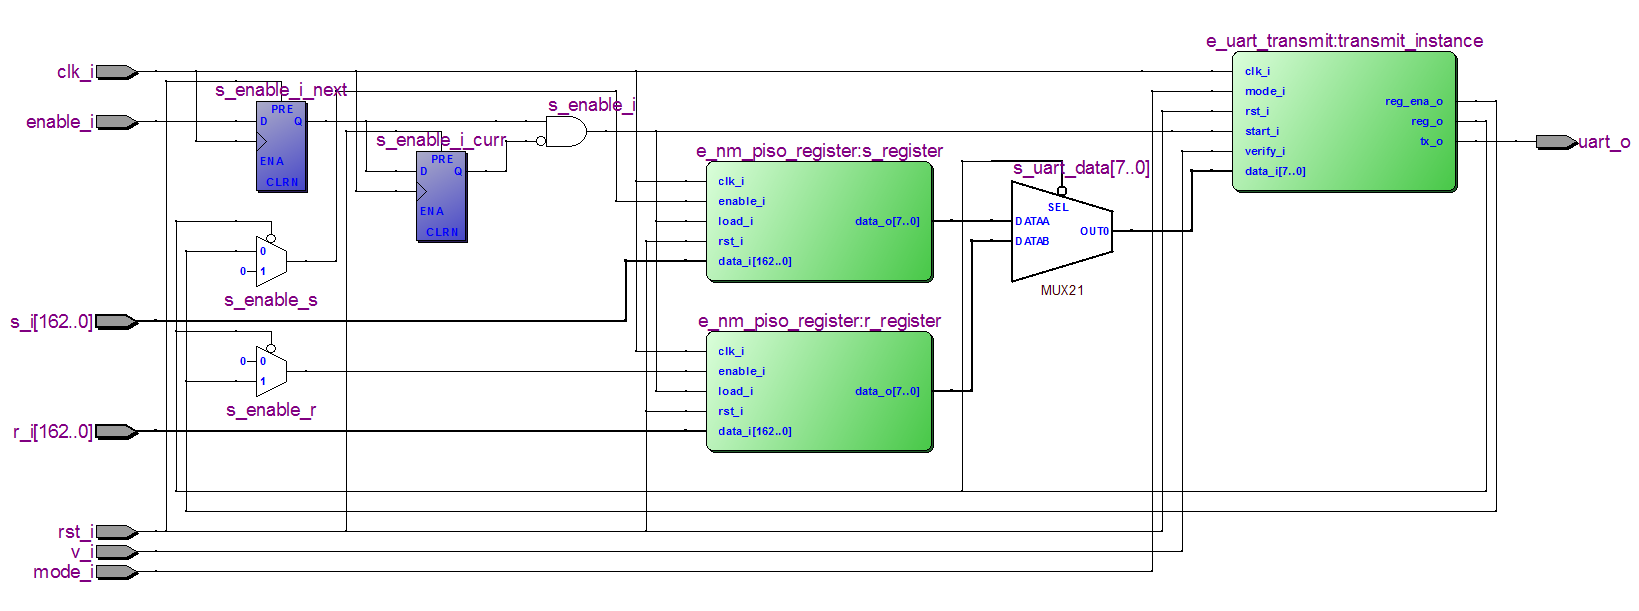
\includegraphics[width=\textwidth]{bilder/uart-transmitter}
	\caption{Ansicht des UART-Transmitter im RTL Viewer}
	\label{fig:uarttx}
\end{figure}

Im Modus Signieren sendet das Modul den in den Registern gespeicherten Punkt $(r, s)$. Beim Verifizieren wird entweder ein Byte Nullen (Signatur passt \textit{nicht} zum Dokument) oder ein Byte Einsen (Signatur gehört zum Dokument) versendet. Der Transmitter instantiiert intern einen Timer, der das Senden am Ausgang Tx in der vor der Synthetisierung eingestellten Baud-Rate taktet. \\



%%%%%%%%%%%%%%%%%%%%%%%%%%%%%%%%%%%%%%%%%%%%%%%%%%%%%%%%%%%%%
\section{Synthese und Pin-Belegung}

Der verwendete FPGA ist ein Baustein der Altera Cyclone II Familie (EP2C35F672C6). Für die Synthetisierung wird das in der Entwicklungsumgebung Quartus II vom selben Hersteller enthaltene Werkzeug verwendet. \\

\begin{table} [h]
	\centering 
	\begin{tabular}{ | p{6cm} | p{3cm} | }
		\hline
		\textbf{Beschreibung} & \textbf{Wert}\\
		\hline
		Ressourcennutzung & 21\% \\
		\hline
		Anzahl Logikelemente & 23,781 / 33,216 ( 72 \% ) \\
		\hline
		Anzahl Register & 15508 \\
		\hline
		Anzahl Pins & 5 / 475 ( 1 \% ) \\
		\hline
	\end{tabular}
	\caption{Ergebnisse der Synthetisierung}
	\label{tab:vhdl-impl-de2}
\end{table}

Abbildung \ref{fig:pins} zeigt die Belegung der verwendeten Pins des Altera DE2 Boardes.

\begin{figure}[H]
	\centering
	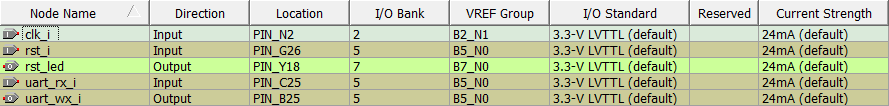
\includegraphics[width=\textwidth]{bilder/pins}
	\caption{Pin-Zuordnung des FPGA}
	\label{fig:pins}
\end{figure}

%!TEX root = ../thesis.tex

\chapter{Messung \& Vergleich} \label{sec:messung}

%%%%%%%%%%%%%%%%%%%%%%%%%%%%%%%%%%%%%%%%%%%%%%%%%%%%%%%%%%%%%
\section{FPGA-Implementierung}
Zur Messungen der Laufzeit werden Daten über die UART-Schnittstelle gesendet und die Zeit gemessen, bis das Ergebnis empfangen wurde. Da das Signieren bzw. Verifizieren, wie in Abschnitt \ref{sec:uartimpl} beschrieben, durch separate Kommandos möglich ist, kann so die Laufzeit pro Funktion ermittelt werden. 
\\ \\
Die Kommunikation mit der FPGA-Implementierung wird über ein selbstgeschriebenes Python-Skript abgewickelt, welches einen zufälligen 163-Bit Hash erzeugt und via UART versendet. Nach dem Empfangen der erzeugten Signatur wird diese erneut zum FPGA geschickt und verifiziert. Dieser Ablauf wird für 1000 Messungen wiederholt und anschließend der Mittelwert gebildet. Die Ergebnisse sind in Tabelle \ref{vhdl-messung} zu finden.
\\
\begin{table}[h]
	\centering 
	\begin{tabular}{ | p{3cm} | p{6cm} | }
		\hline
		\textbf{Funktion} & \textbf{Zeit} \\
		\hline
		Signieren & 77,0 ms \\
		\hline
		Verifizieren & 130,1 ms \\
		\hline
	\end{tabular}
	\caption{Messergebnisse der VHDL-Implementierung}
	\label{vhdl-messung}
\end{table}

Bei den Messergebnissen ist zu beachten, dass diese die Zeit zur Übertragung der Daten beinhalten, die je nach verwendeter Funktion stark variieren können. Für eine exakte Bestimmung der Zeiten bedarf es noch einer Bereinigung der Messergebnisse. Dazu wird rechnerisch ermittelt, wie viel Zeit für die Übetragung benötigt wird und dieser Wert von den gemessenen Zeiten abgezogen. Die serielle Übertragung findet mit einer Geschwindigkeit von 9600 Baud statt. Ein Symbol liegt dadurch für die Signaldauer von 1/9600 Sekunden, also etwa 104$\mu$s, auf der Leitung an. Zusätzlich zu den 8 Daten-Bits werden pro Übertragung noch das Start-Bit und das Stopp-Bit übermittelt. Somit werden Für die 10 Symbole ca. 1,04 ms benötigt. Da die internen Verzögerungen zwischen der UART-Schnittstelle und der ECDSA-Implementierung zu vernachlässigen ist, wird lediglich die UART-Kommunkation berücksichtigt. Dies führt zu den folgenden Messergebnissen:
\\
\begin{itemize}
	\item \textbf{Signieren:}\\
\textit{Senden:} 
1 Byte Modus, 21 Byte Message\\
$\Rightarrow$ 22 Byte * 10 Symbole * 104$\mu$s = 22,92ms\\
\textit{Empfangen:} 
2x21 Byte Punkte der ECC-Funktion\\
$\Rightarrow$ 42 Byte  * 10 Symbole * 104$\mu$s = 43,75ms \\
%\textbf{Nettozeit Signieren} = 123,0ms - 22,92ms - 43,75ms = \textbf{56,3ms}
\textbf{Nettozeit Signieren} = 77,0ms - 22,92ms - 43,75ms = \textbf{10,3ms}
	
	\item \textbf{Verifizieren:}\\
\textit{Senden:}\\
1 Byte Modus, 2x21 Byte ECC-Punkte, 21 Byte Message\\
$\Rightarrow$ 64 Byte * 10 Symbole * 104 $\mu$s = 66,67 ms\\
\textit{Empfangen:}\\
1 Byte für True/False
$\Rightarrow$ 1 Byte  * 10 Symbole * 104 $\mu$s = 1,04 ms \\
%\textbf{Nettozeit Verifizieren} = 74 ms - 66,67 ms - 1,04 ms = \textbf{6,3 ms}\\
\textbf{Nettozeit Verifizieren} = 130,1 ms - 66,67 ms - 1,04 ms = \textbf{62,4 ms}\\
\end{itemize}

Die korrigierten Ergebnisse der Messung werden abschließend dem Simulator-Ergebnis gegenübergestellt: Das Signieren eines 163 Bit Hashes benötigt nur \textbf{23,6 ms} im Simulator, während das Verifizieren \textbf{32,8 ms} benötigt. Beide berechnete Simulationen sind damit mehr als Faktor 2 schneller. Der Grund dafür kann in der Pufferung der verwendeten ``PySerial''-Bibliothek für serielle Schnittstellen in Python sowie an der Puffer-Mechanismen des Betriebssystems liegen. \\

\begin{table}[h]
	\centering 
	\begin{tabular}{ | p{3cm} | p{6cm} | }
		\hline
		\textbf{Funktion} & \textbf{Zeit} \\
		\hline
		Signieren & 10,3 ms \\
		\hline
		Verifizieren & 62,4 ms \\
		\hline
	\end{tabular}
	\caption{Korrigierte Messergebnisse der VHDL-Implementierung}
	\label{vhdl-messung-2}
\end{table}

%%%%%%%%%%%%%%%%%%%%%%%%%%%%%%%%%%%%%%%%%%%%%%%%%%%%%%%%%%%%%
\section{C-Implementierung}
Für die Messung des C-Codes wurde die vorhandene C-Implementierung um Code zum Messen der Funktionen ergänzt und auf einem Rechner mit dem Betriebssystem Linux kompiliert und gestartet. Eine Übersicht der verwendeten Hardware ist in Tabelle \ref{c-impl-hardware} zu finden.

\begin{table}
	\centering 
	\begin{tabular}{ | l | l | }
		\hline
		Bezeichnung & Beschreibung \\
		\hline
		CPU & Intel i5-5200U DualCore (2.20 bis 2.70 GHz, 3MB Cache) \\ 
		RAM & 8GB DDR3L-1600 \\
		HDD & 256GB SSD  \\
		Grafik & Intel® HD 5500 Grafik \\
		OS & Linux \\
		\hline
	\end{tabular}
	\caption{Konfiguration der verwendeten Hardware}
	\label{c-impl-hardware}
\end{table}

Wie bereits bei der VHDL-Implementierung wurden wieder $1000$ Messungen durchgeführt, bei denen im Mittel die Ergebnisse aus Tabelle \ref{c-messung} erzielt wurden.

\begin{table}[h]
	\centering 
	\begin{tabular}{ | p{3cm} | p{6cm} | }
		\hline
		\textbf{Funktion} & \textbf{Zeit} \\
		\hline
		Signieren & 169.1 ms \\
		\hline
		Verifizieren & 340.5 ms \\
		\hline
	\end{tabular}
	\caption{Messergebnisse der C-Implementierung}
	\label{c-messung}
\end{table}

%%%%%%%%%%%%%%%%%%%%%%%%%%%%%%%%%%%%%%%%%%%%%%%%%%%%%%%%%%%%%
\section{Gegenüberstellung \& Bewertung}

Bei den Messergebnissen aus Tabelle \ref{messung-results} ist klar zu erkennen, dass die VHDL-Implementierung je nach Funktion eine Performance-Steigerung zwischen 82 \% - 95 \% aufweist. \\

\begin{table} [h]
	\centering 
	\begin{tabular}{ | p{3cm} | p{2cm} | p{2cm} | p{2cm} | }
		\hline
		 & \textbf{VHDL} & \textbf{C} & \textbf{Gewinn} \\
		\hline
		\textbf{Signieren} & 10,3 ms & 169,1 ms & 94 \% \\
		\hline
		\textbf{Verifizieren} &  62,4 ms & 340,5 ms & 82 \% \\
		\hline
	\end{tabular}
	\caption{Gegenüberstelung der Messergebnisse von der C- und VHDL-Implementierung}
	\label{messung-results}
\end{table}

Bei den Messungen gilt zu berücksichtigen, dass der Performance-Gewinn bereits bei einer geringen Schlüssellänge von 163 Bit erzielt wurde. Da bei einem Erhöhen der Schlüssellänge die Vorteile der Hardware-Implementierung mehr zum Tragen kommen, ist mit weiteren Leistungssteigerungen zu rechnen. Außerdem wurde, wie in Kapitel \ref{sec:impl} beschrieben, lediglich eine triviale VHDL-Implementierung umgesetzt. Durch ein Austauschen der generischen Implementierung durch eine feste Verdrahtung der Bitlängen oder anderen Optimierungen sollen sich weitere Performance-Verbesserungen erzielen lassen.
\\ \\
Abschließend sei noch einmal erwähnt, dass die C-Implementierung eine auf Hardware optimierte Implementierung (Bit-Felder) verwendet. Es ist daher davon auszugehen, dass sich auch die C-Ergebnisse verbessern lassen, indem beispielsweise auf numerische Verfahren zurückgegriffen wird!  

%\begin{figure}[H]
%	\centering
%  \includegraphics[width=1.00\textwidth]{bilder/filename}
%	\caption{caption}
%	\label{label}
%\end{figure}

\chapter{Zusammenfassung \& Ausblick} \label{sec:fazit}



%\chapter{Ausblick}


% Anhang
\chapter{Anhang}

\section{Zustandsautomat im UART-Receiver-Modul} \label{sec:anhang1}

\begin{figure}[thb]
	\centering
  	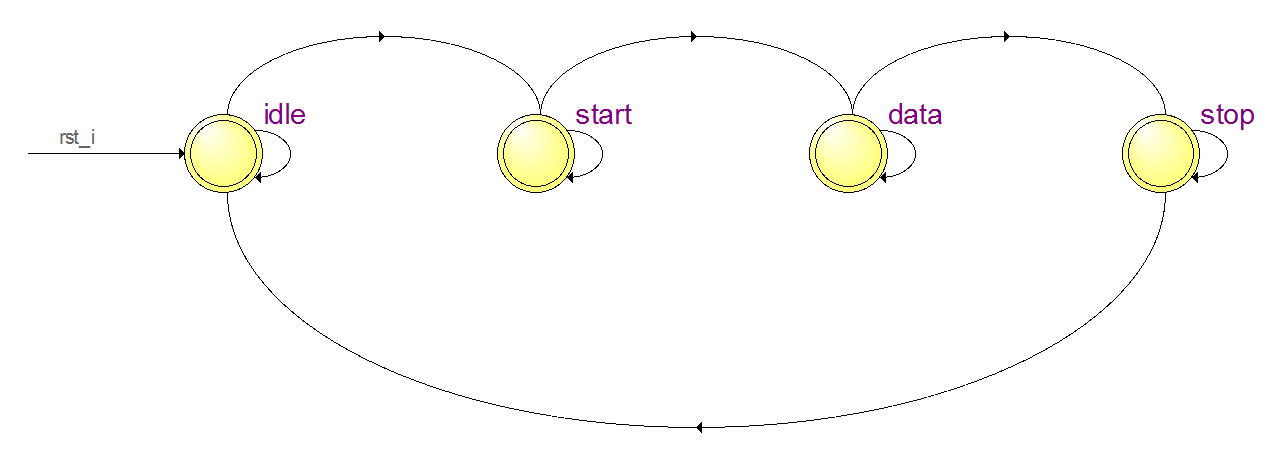
\includegraphics[width=0.8\textwidth]{bilder/uart-receiver-data}
	\caption{Zustandsautomat des Receivers zu Erkennung eines UART-Datenpakets}
	\label{fig:uart-receiver-data}
\end{figure}

\newpage


\pagenumbering{Roman}
\setcounter{page}{5}


\listoffigures
%\lstlistoflistings
%\chapter{Literaturverzeichnis}

\bibliography{thesis} % create with BibTeX

%%!TEX root = ../thesis_main.tex
\chapter{Eidesstattliche Erklärung}
Ich erkl\"are hiermit an Eides statt, dass ich die vorliegende Arbeit selbstst\"andig und ohne Benutzung anderer als der angegebenen Hilfsmittel angefertigt habe; die aus fremden Quellen direkt oder indirekt \"ubernommenen Gedanken sind als solche kenntlich gemacht. Die Arbeit wurde bisher in \"ahnlicher Form keiner anderen Pr\"ufungskommission vorgelegt und auch nicht ver\"offentlicht.

\bigskip
\bigskip
\bigskip
\bigskip
	
   \begin{multicols}{2}
      \raggedright
      Ort, Datum
        
      \raggedleft
      \authorname
      
   \end{multicols}


\end{document}
